\documentclass[twocolumn]{aastex631}
\received{\today}
\shorttitle{APO Proposal}
\graphicspath{{figures/}}

\usepackage{lipsum}
\usepackage{physics}
\usepackage{multirow}
\usepackage{xspace}
\usepackage{natbib}
\usepackage{fontawesome5}
\usepackage{xcolor}
\usepackage{wrapfig}
\usepackage[figuresright]{rotating}

% remove indents in footnotes
\usepackage[hang,flushmargin]{footmisc} 

\newcommand{\todo}[1]{{\color{red}{[TODO: #1}]}}
\newcommand{\needcite}{{\color{magenta}{(needs citation)}}}
\newcommand{\placeholder}[1]{{\color{gray} \lipsum[#1]}}

% custom function for adding units
\makeatletter
\newcommand{\unit}[1]{%
    \,\mathrm{#1}\checknextarg}
\newcommand{\checknextarg}{\@ifnextchar\bgroup{\gobblenextarg}{}}
\newcommand{\gobblenextarg}[1]{\,\mathrm{#1}\@ifnextchar\bgroup{\gobblenextarg}{}}
\makeatother

\begin{document}

\title{{\Large Planetary Radius Valley Investigation}\\\vspace{0.15cm}ASTR 581 APO Proposal}

% affiliations
\newcommand{\UW}{Department of Astronomy, University of Washington, Seattle, WA, 98195}

\author[0000-0001-6147-5761]{Tom Wagg}
\affiliation{\UW}

\correspondingauthor{Tom Wagg}
\email{tomwagg@uw.edu}

\section{Science Justification}
\citep{Christiansen+2018}, \citep{Lopez+2019} \citep{Hardegree-Ullman+2021}, \citep{Acuna+2022}
\placeholder{1-2}


% \begin{figure}
%     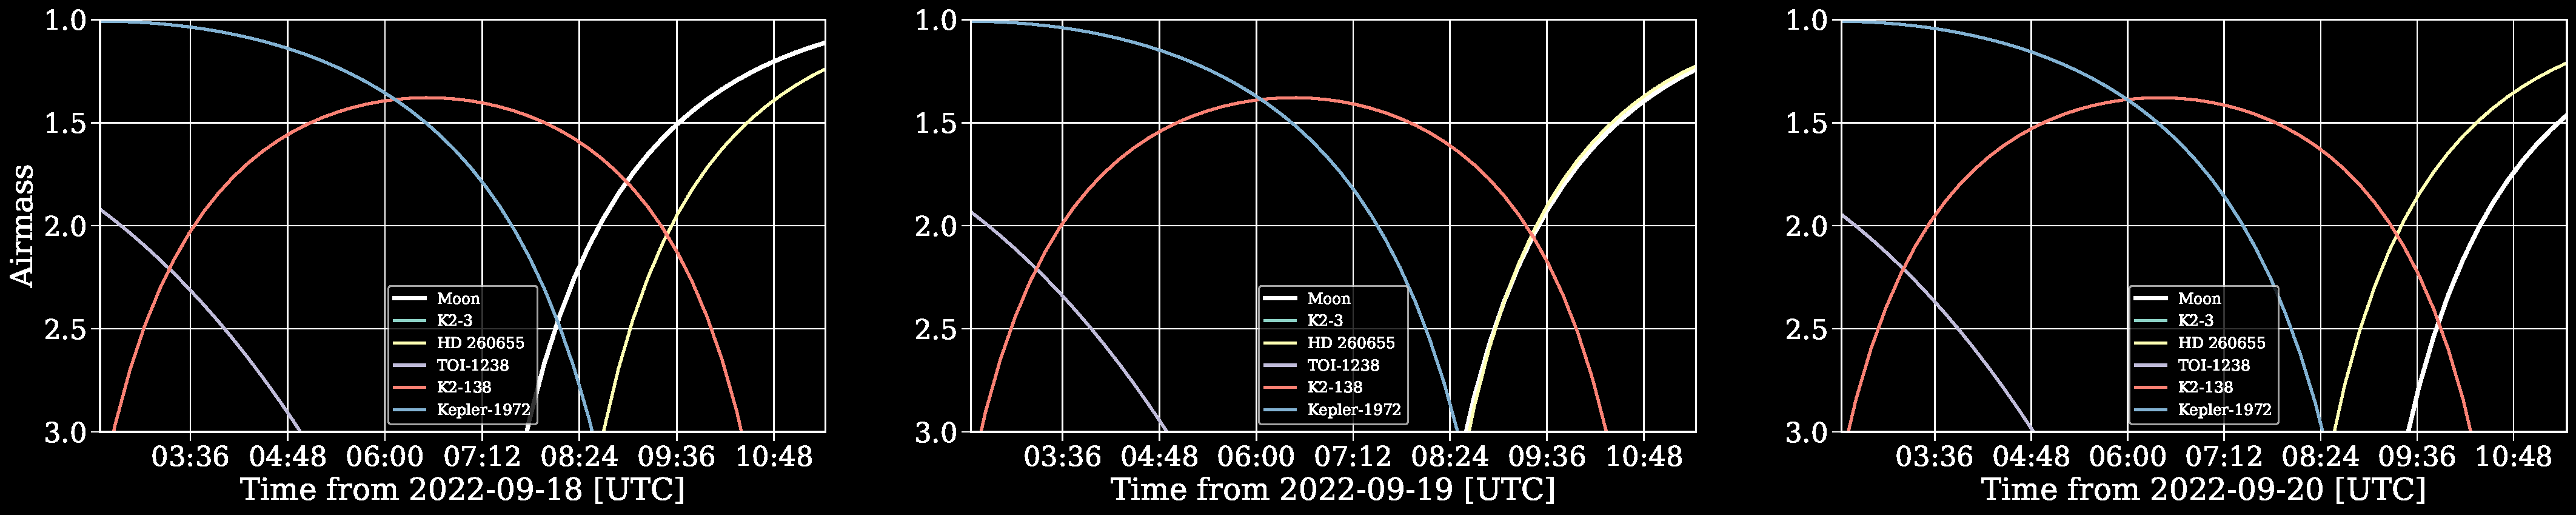
\includegraphics[width=\columnwidth]{potential_systems.pdf}
%     \caption{Airmass over time for different potentially observable multi-transiting systems. Different panels correspond to different observing nights. Shaded grey regions indicate twilight times and sunset.}
% \end{figure}

\section{Proposed Observations}
\begin{figure}[htb]
    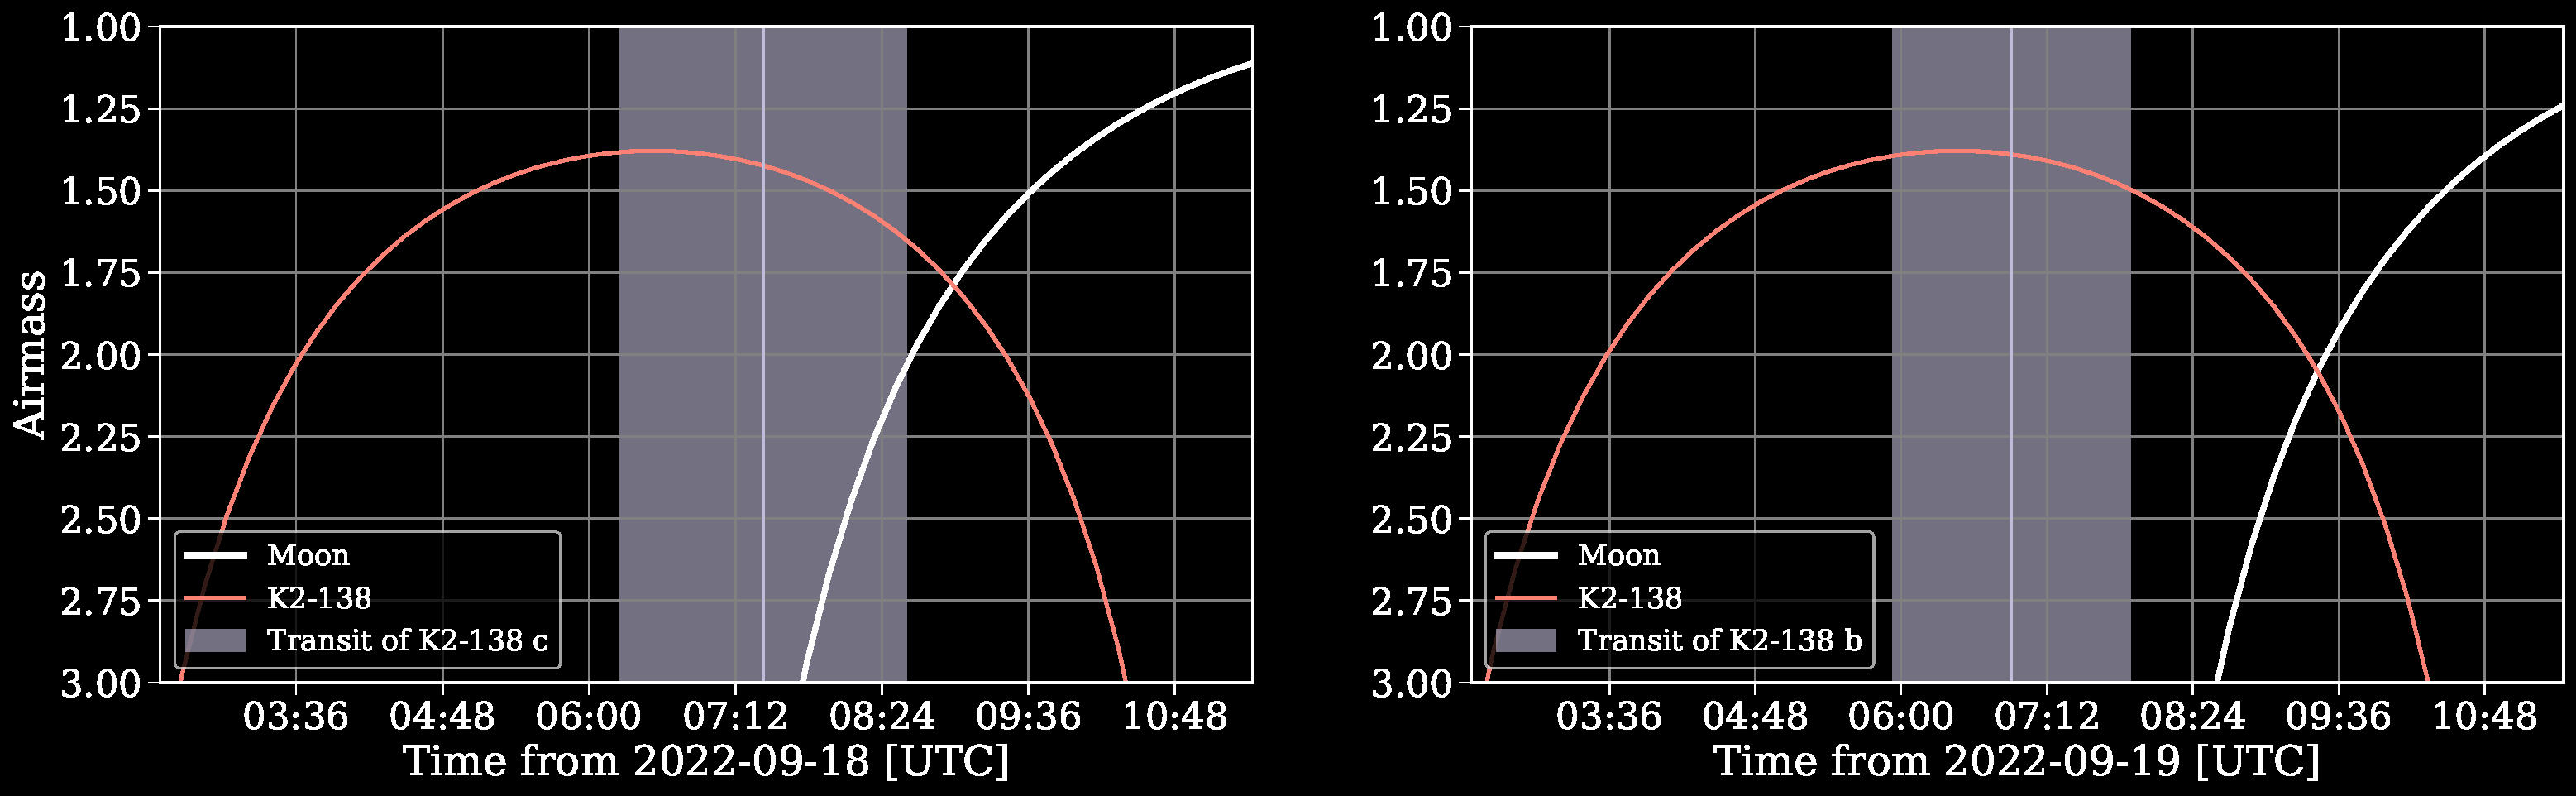
\includegraphics[width=\columnwidth]{observable_transits.pdf}
    \caption{Proposed transit observation for K2-138. Airmass over time for two separate observing nights. Grey shaded regions indicate sunset and twilight times. Orange shaded region indicates transit period and orange line represents the time of mid-transit.}
\end{figure}

We propose to observe two transits of K2-138 on 2022-09-18 and 2022-09-19 by K2-138c and K2-138b respectively using ARCTIC in order to better characterise the lightcurve. In particular, we aim to focus on the ingress and egress of the transit. The transit durations are 1.95 and 2.34 hours respectively and we need to observe the flux for 30 minutes prior to and after the transit. We therefore request two half-nights that include the transits (see Table~\ref{tab:transits}).

We intend to use to narrow-band H-$\alpha$ filter in order to prevent saturation that can occur when using broadband filters with a star of this magnitude\footnote{\url{https://www.apo.nmsu.edu/arc35m/Instruments/ARCTIC/\#3p6}}. We will observe with a cadence of 2 minutes and an exposure time of 3-5 seconds, using the default medium readout time of 25 seconds\footnote{\url{https://www.apo.nmsu.edu/arc35m/Instruments/ARCTIC/\#3p1}}. Since one of the main purposes of these observations is to better characterise the lightcurve and transit timing variations, we will increase the cadence to 30 seconds for 20 minutes around the ingress and egress of the transits, using the fast readout time of 11 seconds (see Table~\ref{tab:settings}).

\begin{table}[htb]
    \centering
    \begin{tabular}{l|c} 
        \hline
        Property & Value \\
        \hline\hline
        Right Ascension & 23h15m47.77s \\
        Declination & $-10^\circ$ $50^\prime$ $59.06^{\prime\prime}$ \\
        V-band Magnitude & 12.25 \\
        Stellar Type & K1V \\
        \hline
    \end{tabular}
    \caption{Properties of the proposed target star KS-138}
    \label{tab:star}
\end{table}

\begin{table}[htb]
    \centering
    \begin{tabular}{l|c|c|c|c} 
        \hline
        Planet & Transit Date & Ingress & Mid-Transit & Egress \\
        \hline\hline
        KS-138c & 2022-09-18 & 05:56 & 06:54 & 07:53 \\
        KS-138b & 2022-09-19 & 06:27 & 07:26 & 08:24 \\
        \hline
    \end{tabular}
    \caption{Transit information for planets around KS-138 in UTC}
    \label{tab:transits}
\end{table}

\begin{table}[htb]
    \centering
    \begin{tabular}{l|c|c} 
        \hline
        \multicolumn{1}{l|}{\multirow{2}{*}{Setting}} & \multicolumn{2}{c}{Value}                                         \\ \cline{2-3} 
\multicolumn{1}{l|}{}                         & \multicolumn{1}{c|}{Regular} & \multicolumn{1}{c}{Ingress/Egress} \\
        \hline\hline
        Exposure Time & 3-5 seconds & 3-5 seconds\\
        Filter & H-$\alpha$ & H-$\alpha$ \\
        Readout time & 25 seconds & 11 seconds \\
        Cadence & 2 minutes & 30 seconds \\
        \hline
    \end{tabular}
    \caption{ARCTIC Settings for observations. We increase use the ARCTIC fast readout time and increase the cadence for 20 minutes around transit ingress and egress in order to better characterise transit timing variations.}
    \label{tab:settings}
\end{table}

\bibliographystyle{aasjournal}
\bibliography{proposal}{}

\end{document}